\begin{chapter}{Control}

    % robust linear control: https://inst.eecs.berkeley.edu/~ee127/sp21/livebook/l_sdp_apps_stability.html
    % AA203 Examples: https://github.com/StanfordASL/AA203-Examples
    % multi target tracking
        % MATLAB: https://www.mathworks.com/videos/sensor-fusion-part-5-how-to-track-multiple-objects-at-once-1569411395828.html 
        % potentially good: https://stonesoup.readthedocs.io/en/v0.1b9/auto_tutorials/06_DataAssociation-MultiTargetTutorial.html
    % Learning convex control policies https://stanford.edu/~boyd/papers/pdf/l4dc_cocp_talk.pdf
    % "" but longer: https://stanford.edu/~boyd/papers/pdf/learning_cocps.pdf
    % real time multiple object tracking for autonomous navigation: https://cs231n.stanford.edu/reports/2017/pdfs/630.pdf
    % Learning to track: https://cvgl.stanford.edu/papers/xiang_iccv15.pdf
    
    \section{Overview}

    % Need to add AA203 overview to this

    \begin{figure}[h!]
        \centering
        \begin{forest}
            for tree={
                grow=east,
                parent anchor=east,
                child anchor=west,
                edge path={
                    \noexpand\path [draw, \forestoption{edge}]
                    (!u.parent anchor) -- +(5pt,0) |- (.child anchor)\forestoption{edge label};
                },
                l sep+=10pt,
                s sep+=10pt,
                anchor=west,
                align=center
            }
            [Control
                [Passive\\(Optimal Design)]
                [Active
                    [Open Loop]
                    [Closed Loop]
                ]
            ]
        \end{forest}
        \caption{Control Strategies}
        \label{fig:control_tree}
    \end{figure}

    \begin{figure}[h!]
        \centering
        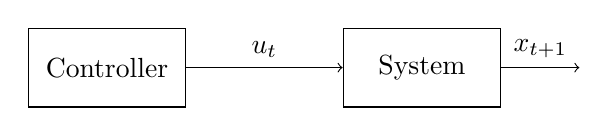
\begin{tikzpicture}[auto, node distance=2cm]
            % Nodes
            \node [draw, rectangle, minimum width=2cm, minimum height=1cm] (control) {Controller};
            \node [draw, rectangle, minimum width=2cm, minimum height=1cm, right of=control, node distance=4cm] (system) {System};
            
            % Arrows
            \draw [->] (control) -- node[above] {$u_t$} (system);
            \draw [->] (system) -- node[above] {$x_{t+1}$} ++(2cm, 0);
    
        \end{tikzpicture}
        \caption{Open Loop Control Strategy}
        \label{fig:block_diagram}
    \end{figure}

    Source: Control bootcamp (Brunton)
    \begin{itemize}
        \item (Dynamical Systems) Systems of ODEs describing state of system has been a successful modeling framework.
        \item Often want to actively make changes to the system. 
        \item In control theory, you have a dynamical system of interest, you write down the system of equations 
        which describes the behavior of the system, and then you create a control theory to create a more ``desireable''
        system behavior.
        \item Passive control (Boyd would call optimal design): design an upfront solution (ex: minimizing drag on a truck)
        \item Active control: pump energy into the system to actively manipulate its behavior.
    \end{itemize}

    \noindent Active Control
    \begin{itemize}
        \item Open Loop
    \end{itemize}

    % \section{Optimal Design}

    % % non stochastic closed loop control
    % \noindent~\cite*{boyd_convex_optimization} \textbf{Exercise 4.17}. \textit{Optimal Activity Levels}.We consider an alternative control application: central planning of some economic activity. It's straightforward to formulate the problem as

    % \[
    % \begin{array}{lll}
    % \text{maximize} \; & \sum_{j=1}^{n}r_j(x_j) & \\
    % \text{subject to} & Ax \preceq c^{\text{max}} &  \\
    % & x \succeq 0. \; & 
    % \end{array}\]
    % However, while the revenue function is a piecewise-linear concave function of the activity
    % level (as stated in the text)

    % \[ r_j(x_j) = \begin{cases}
    %     p_j x_j & 0 \le x_j \le q_j \\
    %     p_j q_j + p_j^{\text{disc}}(x_j - q_j) & x_j \ge q_j,
    % \end{cases}\]
    % this 

    \section{Basic Examples}

    ~\cite{boyd_convex_optimization} \textbf{Exercise 4.16}. \textit{Minimum fuel optimal control}.
    Consider the LTI dynamical system with state $x_t \in \mathbf{R}^n$, $t = 0, \ldots, N$, and actuator
    or input signal $u_t \in \mathbf{R}$, for $t = 0, \ldots, N-1$. The dynamics of the system are governed by the
    linear recurrence
    \[x_{t+1} = Ax_t + bu_t, \quad t=0, \ldots N-1,\]
    where $A \in \mathbf{R}^{m \times n}$ and $b \in \mathbf{R}^n$ are given. Assume the initial state is $x_0 = 0$.
    The \textit{minimum fuel optimal control problem} is to choose the inputs $u_0, \ldots u_{N-1}$ so as to
    minimize the total fuel consumed, which is given by
    \[F = \sum_{t=0}^{N-1}f(u_t),\]
    subject to the constraint that $x_N = x_{\text{des}}$, where $N$ is the (given) time horizon and
    $x_{\text{des}} \in \mathbf{R}^n$ is the (given) desired final or target state. The function $f: \mathbf{R} \to \mathbf{R}$
    is the \textit{fuel use map} for the actuator, and gives the amount of fuel used as a function of the actuator signal amplitude.
    In this problem we use
    \[f(a) = \begin{cases}
        \left| a \right| & \left| a \right| \le 1 \\
        2 \left| a \right| - 1 & \left| a \right| > 1.
        \end{cases}\]
    Formulate the minimum fuel control problem as an LP. 

    \vspace{.1cm}
    \noindent \textbf{Response.}
        Firstly, a few notes about the problem itself:
        \begin{itemize}
            \item ~\cite*{actuator_youtube} What is an actuator (broadly)?
                \begin{itemize}
                    \item A device that makes something move or operate.
                    As a trivial example, an actuator moves the sliding doors at a grocery store.
                    \item Two types: straight line movement (linear) and circular movement (rotary).
                    \item An actuator converts a source of energy into a physical, mechanical motion.
                    A silly example of this: a handwheel can be used to feed energy into a rotary actuator.
                    In industrial applications, there are three typical sources of energy: \textit{Electric} uses electricty (duh),
                    \textit{hydraulic} use a variety of liquids, \textit{pneumatic} are operated by compressed air.
                    \item Common industrial actuators are electric motors, hydraulic motors, and pneumatic control valves.
                    \item Example use of a pneumatic actuator: ``PLC analog output card* produces a 4-20 mA current to move the 
                    valve from fully open to fully closed. The 4-20 mA current will be converted to pneumatic pressure, which
                    becomes the source of energy to operate the actuator.''
                    \item *A Programmable Logic Controller (PLC) analog output card is a component
                    used to convert digital signals from the PLC's processor into analog signals (digital-to-analog conversion, DAC that can
                    be used to control external devices.
                \end{itemize}
            \item Actuator in this problem.
                \begin{itemize}
                    \item $u_t$ is a scalar valued signal that directly affects the state
                    of our system of interest (since it's in the linear recurrence equation).
                    \item Physically, this signal is being used to direct the actuator, which
                    in turn is turning energy into mechanical motion.
                    \item Therefore, the fuel use map for the actuator is a mathematical
                    relation between the amplitude of the signal directing the actuator and
                    the fuel being used. In other words, we can imagine a larger actuator
                    signal corresponds to greater actuator motion, and in this instance,
                    the source of energy needed to produce this motion is ``fuel.''
                \end{itemize}
        \end{itemize}
    % perhaps note that once you establish techniques, you'll stop being explicit with formulations.
     Naive formulation of this problem 
    \[\begin{array}{lll}
    \text{minimize} \; & \sum_{t=0}^{N-1} f(u_t) & \\
    \text{subject to} & x_{t+1} = Ax_t + bu_t \; & t=0, \ldots, N-1 \\
    & x_0 = 0, \quad x_{N} = x_{\text{des}}.
    \end{array}\]
    
    Consider the graph of the fuel use map~\ref{fig:fuel-map}

    % Important/Helpful to map this back to 4.11
    % Actually, how would you map this to ||Ax-b||_1 approximation
    \begin{figure}[h]
        \centering
        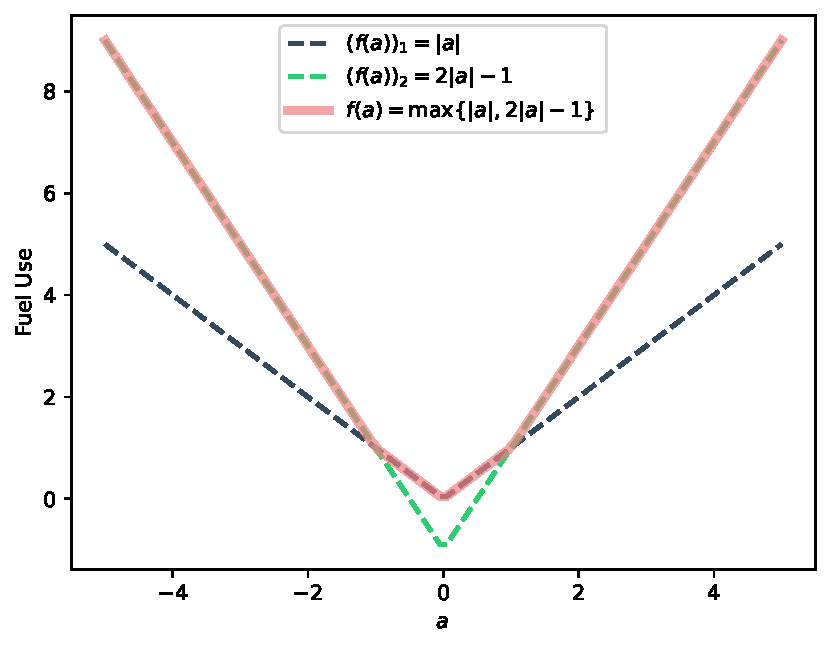
\includegraphics[width=\linewidth]{examples/cvx-ch4/actuator_fuel-use.pdf}
        \caption{Actuator Fuel Use Map.}
        \label{fig:fuel-map}
    \end{figure}

    \[\begin{array}{lll}
        \text{minimize} \; & \sum_{t=0}^{N-1} \max \left\{ \left| u_t \right|, 2 \left| u_t \right| - 1 \right\} & \\
        \text{subject to} & x_{t+1} = Ax_t + bu_t \; & t=0, \ldots, N-1 \\
        & x_0 = 0, \quad x_{N} = x_{\text{des}}.
        \end{array}\]

    \[\begin{array}{lll}
        \text{minimize} \; & \bm{1}^T t & \\
        \text{subject to} & x_{t+1} = Ax_t + bu_t \; & t=0, \ldots, N-1 \\
        & x_0 = 0, \quad x_{N} = x_{\text{des}}, & \\
        & \max \left\{ \left| u_i \right|, 2 \left| u_i \right| - 1 \right\} \le t_i, & i = 0, \ldots, N-1
        \end{array}\]

    \[\begin{array}{lll}
        \text{minimize} \; & \bm{1}^T t & \\
        \text{subject to} & x_{t+1} = Ax_t + bu_t \; & t=0, \ldots, N-1 \\
        & x_0 = 0, \quad x_{N} = x_{\text{des}}, & \\
        & \left| u_i \right| \le t_i, & i = 0, \ldots, N-1 \\
        & 2 \left| u_i \right| - 1 \le t_i & i = 0, \ldots, N-1 \\
        \end{array}\]
    
    \[\begin{array}{lll}
    \text{minimize} \; & \bm{1}^T t & \\
    \text{subject to} & x_{t+1} = Ax_t + bu_t \; & t=0, \ldots, N-1 \\
    & x_0 = 0, \quad x_{N} = x_{\text{des}}, & \\
    & y_i \le t_i, & i = 0, \ldots, N-1 \\
    & 2 y_i - 1 \le t_i & i = 0, \ldots, N-1 \\
    & \left| u_i \right| \le y_i & i = 0, \ldots, N-1 \\
    \end{array}\]
    Important/helpful to remeber the definition of absolute value: $\left| a \right| = \max\{a, -a\}$

    \[\begin{array}{lll}
        \text{minimize} \; & \bm{1}^T t & \\
        \text{subject to} & x_{t+1} = Ax_t + bu_t \; & t=0, \ldots, N-1 \\
        & x_0 = 0, \quad x_{N} = x_{\text{des}}, & \\
        & y_i \le t_i, & i = 0, \ldots, N-1 \\
        & 2 y_i - 1 \le t_i & i = 0, \ldots, N-1 \\
        & -y_i \le u_i \le y_i & i = 0, \ldots, N-1 \\
        \end{array}\]
    Write more compactly as

    \[\begin{array}{lll}
        \text{minimize} \; & \bm{1}^T t & \\
        \text{subject to} & x_{t+1} = Ax_t + bu_t \; & t=0, \ldots, N-1 \\
        & x_0 = 0, \quad x_{N} = x_{\text{des}}, & \\
        & y \preceq t & \\
        & 2y - \bm{1} \preceq t & \\
        & -y \preceq u \preceq y_i & 
        \end{array}\]
    Still not ideal form because of the linear recurrence. Use control theory result.
    
    \begin{figure}[h]
        \centering
        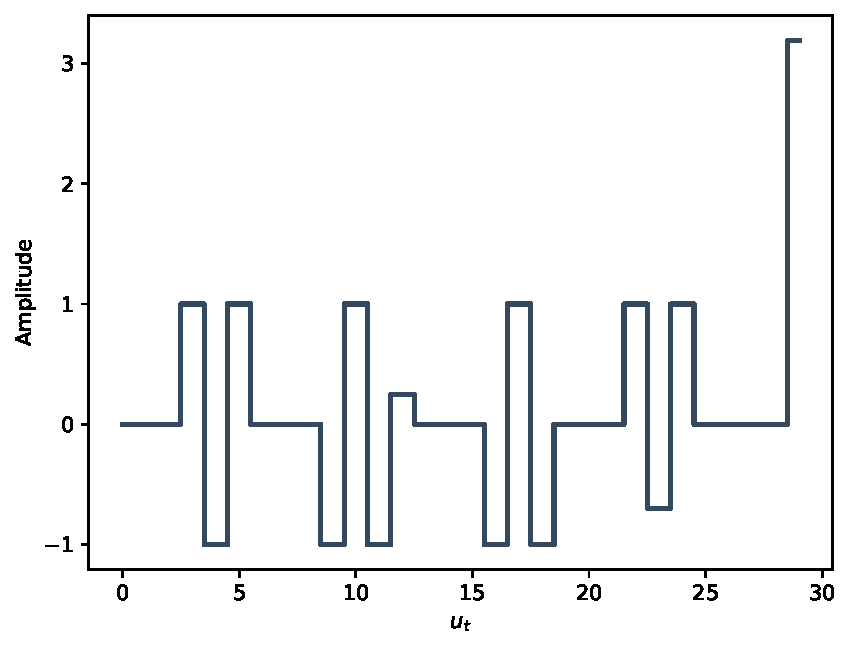
\includegraphics[width=\linewidth]{examples/cvx-ch4/4-16_min-fuel.pdf}
        \caption{Minimum fuel actuator signal.}
        \label{fig:4-16_min-fuel}
    \end{figure}
    
    \vspace*{.5cm}

    \section{Model Predictive Control}

    % Fast MPC: https://web.stanford.edu/~boyd/papers/fast_mpc.html

    \subsection{Overview and Basic Formulations}

    \subsection{Examples}

    % mention that this is a pre real MPC example: no stochasticity
    % list out different variations of MPC

    \subsubsection*{Almost MPC}
    We apply MPC to the following output tracking example. The purpose of this exercise is simply to show
    how sequentially solving receeding horizon problems can converge to the agnostic control problem (where
    the problem is solved with full access to the desired output) as the horizon is increased.
    Note that this example \textbf{does not} demonstrate the power of using MPC in a stochastic setting.

    \noindent~\cite{EE364b} \textbf{HW7 Q1.} \textit{MPC for output tracking}. Consider the linear dynamical system
    \[x_{t+1} = Ax_t + Bu_t, \quad y_t = Cx_t, \quad t = 0, \ldots, T-1,\]
    with state $x_t \in \mathbf{R}^n$, input $u_t \in \mathbf{R}^m$, and output $y_t \in \mathbf{R}^p$.
    The matrices $A$ and $B$ are known, and $x_0=0$. The goal is to choose the input sequence $u_1, \ldots, u_t$
    to minimize the output tracking cost
    \[J_{\text{output}} = \sum_{t=1}^{T}\left\lVert y_t - y_t^{\text{des}} \right\rVert_{2}^2,\]
    subject to $\left\lVert u_t \right\rVert_{\infty} \le U^{\text{max}}, \, t=0, \ldots, T-1$. \\
    For the remainder of this problem we work with the specific problem instance with associated data
    \[A = \begin{bmatrix}
        1 & 1 & 0 \\ 0 & 1 & 1 \\ 0 & 0 & 1
    \end{bmatrix}, \quad
    B = \begin{bmatrix}
        0 \\ 0.5 \\ 1
    \end{bmatrix}, \quad
    C = \begin{bmatrix}
        -1 & 0 & 1
    \end{bmatrix},\]
    $T=100$, and $U^{\text{max}} = 0.1$. The desired output trajectory is given by

    \[y^{\text{des}}_t = \begin{cases}
        0 & t < 30, \\
        10 & 30 \le t < 70 \\
        0 & t \ge 70.
    \end{cases}\]
    (a) Find the optimal input $u^*$ and the associated optimal cost $J^*$.
    
    \vspace{.1cm}
    % is it a linear quadratic tracking problem? What about l_inf constraint?
    \noindent \textbf{Response.} This is simply a \textit{linear} (in the dynamics) \textit{time-invariant quadratic tracking} problem.
    Instead of doing a theoretical analysis of controllability, etc., we can determine the feasibility
    of the control problem by formulating and attempting to solve the following convex optimization problem:
    \[\begin{array}{lll}
    \text{minimize} \; & J_{\text{output}} = \sum_{t=1}^{100}\left\lVert Cx_t - y_t^{\text{des}} \right\rVert_{2}^2 & \\
    \text{subject to} & \left\lVert u_t \right\rVert_{\infty} \le 0.1, \quad x_{t+1} = Ax_t + Bu_t, \; \quad t = 0, \ldots, 99 & \\
    &x_0 = 0,
    \end{array}\]
    (with the provided data for $A$, $B$, $C$, and $y^{\text{des}}$, of course.) Using CVXPY, we obtain the optimal cost 
    $J_{\text{outout}}^{*} = 112.4157$.

    \vspace{.1cm}
    \noindent (b) \textit{Rolling look-ahead}. Now consider the input obtained using an MPC-like method
    where at time $t$, we find the values of $u_t, \ldots, u_{t+N-1}$ that solve the following convex optimization
    problem

    \[\begin{array}{lll}
        \text{minimize} \; & J_{\text{output}} =  \sum_{\tau=t+1}^{t+N}\left\lVert Cx_\tau - y_\tau^{\text{des}} \right\rVert_{2}^2 & \\
        \text{subject to} & \left\lVert u_\tau \right\rVert_{\infty} \le 0.1, \quad x_{\tau+1} = Ax_\tau + Bu_\tau, \; \quad \tau = t, \ldots, t + N - 1 & \\
        &x_0 = 0.
        \end{array}\]
    The value $N$ is the amount of \textit{look-ahead}, since it dictates how much of the future of the desired
    output signal we are allowed to access when we decide on the current input.\\
    Find the input signal for look-ahead values $N=8$, $N=10$, and $N=12$. Compare the cost $J_{\text{output}}$
    obtained in these three instances to the optimal cost $J_{\text{output}}^{*}$ found in part (a).
    
    \vspace{.1cm} 
    \noindent \textbf{Response.} The Python code used to solve this problem can be found in these note's associated examples folder under 364b,
    so it is omitted here. The cost obtained by applying MPC with 
    \begin{itemize}
        \item $N = 8$ is $379.634$,
        \item $N = 10$ is $128.13$,
        \item and $N=12$ is $123.62$.
    \end{itemize}
    Figure~\ref{fig:364-hw7-traj-out} shows the output trajectories for $N=8$, $N=10$, $N=12$,
    the optimal output trajectory, and the desired output trajectory.

    \begin{figure}[h]
        \centering
        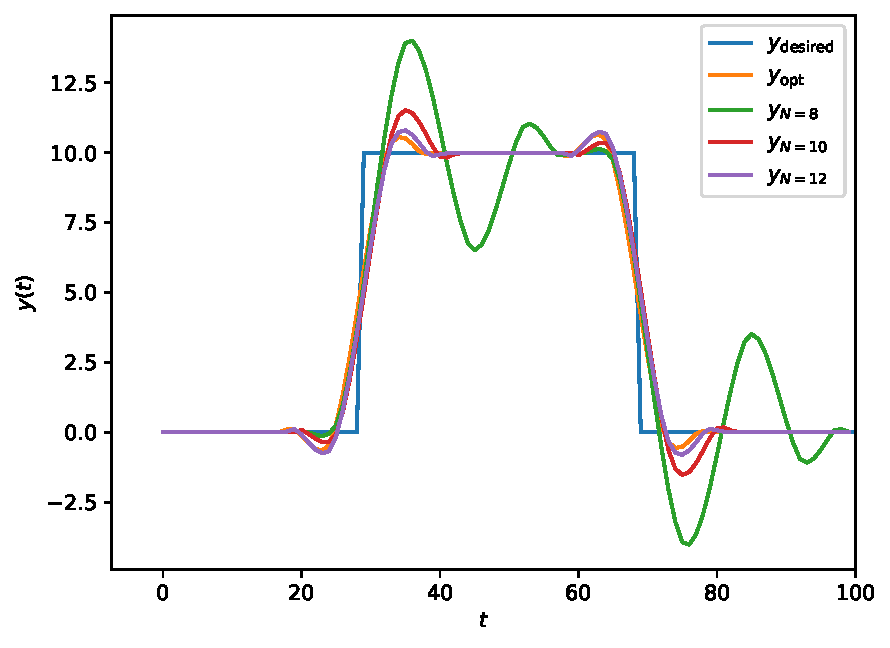
\includegraphics[width=\linewidth]{examples/364b/364b_mpc_output.pdf}
        \caption{Output Trajectories.}
        \label{fig:364-hw7-traj-out}
    \end{figure}
    
\end{chapter}